\documentclass[unknownkeysallowed]{beamer}
\mode<presentation>
{
%  \usetheme{AnnArbor}
%  \usetheme{Dresden}
%  \usetheme{Montpellier}
%  \usetheme{Antibes}
%  \usetheme{Frankfurt}
%  \usetheme{PaloAlto}
%  \usetheme{Bergen}
%  \usetheme{Boadilla}
%  \usetheme{Goettingen}
%  \usetheme{Pittsburgh}	%!!
%  \usetheme{Berkeley}
%  \usetheme{Hannover}
%  \usetheme{Rochester}		%!!!
%  \usetheme{Berlin}
%  \usetheme{Ilmenau}
%  \usetheme{Singapore}
  \usetheme{Boadilla}		%viel platz
%  \usetheme{JuanLesPins}
%  \usetheme{Szeged}		%!
%  \usetheme{boxes}
%  \usetheme{Luebeck}
%  \usetheme{Warsaw}
%  \usetheme{Copenhagen}
%  \usetheme{Madrid}
%  \usetheme{Darmstadt}
%  \usetheme{Malmoe}
%  \usetheme{default}
%  \usetheme{JuanLesPins}

%  \usetheme{Marburg}


%\usefonttheme{professionalfonts}
%	default | professionalfonts | serif |
%	structurebold | structureitalicserif |
%	structuresmallcapsserif
%\useinnertheme{rounded}
%	circles | default | inmargin |
%	rectangles | rounded

%  \setbeamercovered{transparent}
  % oder auch nicht
\usecolortheme{rose}


\definecolor{uaf yellow}{cmyk}{0,0.16,1,0} % official UAF yellow
\definecolor{light yellow}{cmyk}{0.01,0,0.16,0}
\definecolor{uaf blue}{cmyk}{1,0.66,0,0.02} % official UAF blue
\definecolor{light blue}{cmyk}{0.22,0.11,0,0}
\definecolor{arsc blue}{HTML}{005496}
\definecolor{arsc red}{HTML}{a20a42}
\definecolor{arsc green}{HTML}{009a82}
\definecolor{light gray}{HTML}{777777}

  %navigation aus, klaut nur platz
  \setbeamertemplate{navigation symbols}{}
% Reset title background to default
%\setbeamertemplate{title page}[default]
\setbeamercolor{title}{bg=}
\setbeamercolor{frametitle}{bg=uaf blue, fg=white}
\setbeamercolor{institute}{fg=white}
\setbeamercolor{date}{fg=white}
\setbeamercolor{block}{bg=}
%\setbeamercolor{title}{fg=black}

% Reset block background to default
%\setbeamertemplate{blocks}[default]
%\setbeamercolor{block title}{bg=}
%\setbeamercolor{block body}{bg=}

\beamertemplatenavigationsymbolsempty  
\setbeamertemplate{blocks}[rounded][shadows=false]

\useinnertheme{circles}

}
\usepackage[latin1]{inputenc}
\usepackage{latexsym}
\usepackage{amsfonts}
%\usepackage{natbib}
\usepackage{fancyhdr}
\usepackage{graphicx}
%\usepackage{subfigure}
% oder was auch immer
\usepackage{grffile}
\usepackage{pgf}
\usepackage{tikz}

\usepackage{listings}

\usepackage{times}
\usepackage[T1]{fontenc}
%\usepackage{appendixnumber}
% Oder was auch immer. Zu beachten ist, das Font und Encoding passen
% m�ssen. Falls T1 nicht funktioniert, kann man versuchen, die Zeile
% mit fontenc zu l�schen.

\hypersetup{
    bookmarks=true,         % show bookmarks bar?
    unicode=false,          % non-Latin characters in Acrobat's bookmarks
    pdftoolbar=true,        % show Acrobat's toolbar?
    pdfmenubar=true,        % show Acrobat's menu?
    pdffitwindow=false,     % window fit to page when opened
    pdfstartview={FitH},    % fits the width of the page to the window
    pdftitle={My title},    % title
    pdfauthor={Author},     % author
    pdfsubject={Subject},   % subject of the document
    pdfcreator={Creator},   % creator of the document
    pdfproducer={Producer}, % producer of the document
    pdfkeywords={keyword1} {key2} {key3}, % list of keywords
    pdfnewwindow=true,      % links in new window
    colorlinks=false,       % false: boxed links; true: colored links
    linkcolor=red,          % color of internal links
    citecolor=green,        % color of links to bibliography
    filecolor=magenta,      % color of file links
    urlcolor=cyan           % color of external links
}

\title[PAG]% (optional, nur bei langen Titeln n�tig)
{GEOS 436 / 636\\
Programming and Automation for Geoscientists\\[20pt]
-- Week 08: Unix -- Shell --
}

\author[Grapenthin]% (optional, nur bei vielen Autoren)
{Ronni Grapenthin\\
rgrapenthin@alaska.edu\\
Elvey 413B\\
x7682}
% - Namen m�ssen in derselben Reihenfolge wie im Papier erscheinen.
% - Der \inst{?} Befehl sollte nur verwendet werden, wenn die Autoren
%   unterschiedlichen Instituten angeh�ren.

\institute[UAF] % (optional, aber oft n�tig)
{}
% - Der \inst{?} Befehl sollte nur verwendet werden, wenn die Autoren
%   unterschiedlichen Instituten angeh�ren.
% - Keep it simple, niemand interessiert sich f�r die genau Adresse.

% - Namen m�ssen in derselben Reihenfolge wie im Papier erscheinen.
% - Der \inst{?} Befehl sollte nur verwendet werden, wenn die Autoren
%   unterschiedlichen Instituten angeh�ren.

% - Der \inst{?} Befehl sollte nur verwendet werden, wenn die Autoren
%   unterschiedlichen Instituten angeh�ren.
% - Keep it simple, niemand interessiert sich f�r die genau Adresse.

\date[]{}

% - Volle oder abgek�rzter Name sind m�glich.
% - Dieser Eintrag ist nicht f�r das Publikum gedacht (das wei�
%   n�mlich, bei welcher Konferenz es ist), sondern f�r Leute, die diese
%   Folien sp�ter lesen.

%\AtBeginSection[]
%{
%  \begin{frame}<beamer>
%    \frametitle{Outline}
%    \tableofcontents[currentsection,currentsubsection]
%  \end{frame}
%}

% Falls Aufz�hlungen immer schrittweise gezeigt werden sollen, kann
% folgendes Kommando benutzt werden:

%\beamerdefaultoverlayspecification{<+->}

%%switch on to have only frame numbers
\setbeamertemplate{footline}[frame number]

\defbeamertemplate*{title page}{customized}[1][]
{
		\begin{tikzpicture}
			\node[text width=\textwidth,
				fill=gray!70, 
				fill opacity=0.75,
				text opacity=1,
				rounded corners = 10pt,
				inner sep=2pt]{
				\begin{center}	
			  \usebeamerfont{title}{\bf \usebeamercolor[fg]{title} \inserttitle}
			  \par
			  \usebeamerfont{subtitle}\insertsubtitle\par
			  \bigskip
			  \usebeamerfont{author}\insertauthor\par
			  \bigskip
			  \usebeamerfont{institute}\insertinstitute\par
			  \bigskip
			  \usebeamerfont{date}\insertdate\par
			  \end{center}
			  };
	\end{tikzpicture}		  
%	\vspace{0.4cm}\usebeamercolor[fg]{titlegraphic}\inserttitlegraphic 
%	\begin{flushright}
%	\vspace{-1.25cm}\includegraphics[width=2cm]{../moore_logo_transp.png}\vspace{5cm}
%	\end{flushright}
}

\begin{document}

\lstset{numbers=left, numberstyle=\tiny, stepnumber=2, basicstyle=\ttfamily, numbersep=5pt, xleftmargin=10pt}

\setbeamertemplate{background}{\includegraphics[width=\paperwidth]{/home/roon/Pictures/rooftop_initial.jpg}}

	\begin{frame}
	\begin{center}
		\titlepage
	\end{center}
	\end{frame}

\setbeamertemplate{background}{}

\begin{frame}
\frametitle{}
%	\vspace{2cm}
	\begin{center}
		Is there a computer environment that 
		makes it \emph{easy} to automate
		processes??$^{*}$
	\end{center}
	\vspace{4cm}
	{\tiny {\color{gray}$^{*}$hint: YES!!!!}}
\end{frame}

\begin{frame}
	\frametitle{Unix Philosophy}
	\vspace{-0.25cm}
	\begin{itemize}
		\item minimalist
		\item modular
		\item robust
		\item funky user interface (the shell)
	\end{itemize}
	Peter Salus:
	\begin{itemize}
		\item Write programs that do one thing and do it well.
		\item Write programs to work together.
		\item Write programs to handle text streams, because that is a universal interface.
	\end{itemize}

\end{frame}

\begin{frame}
	\frametitle{How do I get it?}
	\begin{itemize}
		\item Unix/Linux - comes with the package (Linux is a free Unix)
		\item Mac OS - derived from Unix; use Terminal.app
		\item Windows - various emulators (e.g., VirtualBox)
		\item We'll use a browser-based interface (JupyterLab) to ensure a homogeneous setup
	\end{itemize}
\end{frame}


\begin{frame}
	\frametitle{Shell}
	\begin{center}
		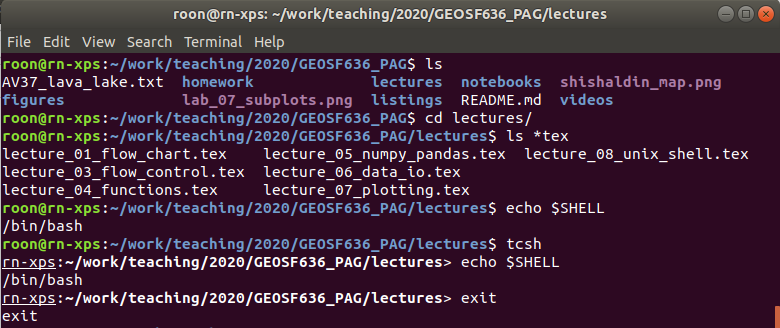
\includegraphics[width=\textwidth]{../figures/terminal.png}
	\end{center}

	\begin{itemize}
		\item Text-based user interface
		\item Interpreter of your commands
		\item Most popular shells: {\tt bash, (t)csh}
		\item Defines your working environment
	\end{itemize}
\end{frame}

\begin{frame}
	\frametitle{Shell Commandline Anatomy}
	\begin{center}
		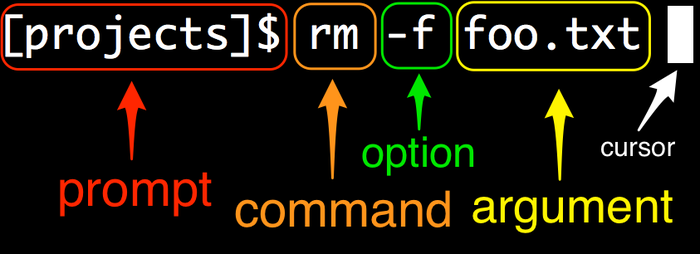
\includegraphics[width=0.75\textwidth]{../figures/shell_cmdline_anatomy.png}
	\end{center}
	\begin{flushright}
		\tiny{\emph{\url{https://www.learnenough.com/command-line-tutorial/basics}}}
	\end{flushright}
	\begin{center}
	(prompt will differ)
	\end{center}
\end{frame}


\begin{frame}
	\frametitle{Command Anatomy}
	\begin{center}
		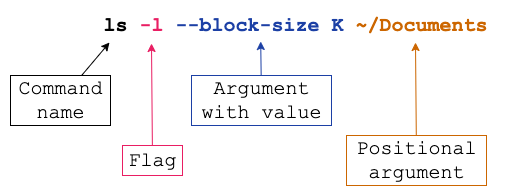
\includegraphics[width=0.5\textwidth]{../figures/shell_command-line-arguments-ls.png}
	\end{center}
	\begin{flushright}
		\tiny{\emph{\url{https://betterdev.blog/command-line-arguments-anatomy-explained}}}
	\end{flushright}
\end{frame}

\begin{frame}[fragile=singleslide]
	\frametitle{Command Anatomy: man-pages}
	\verb|$>man mkdir|
	\begin{center}
		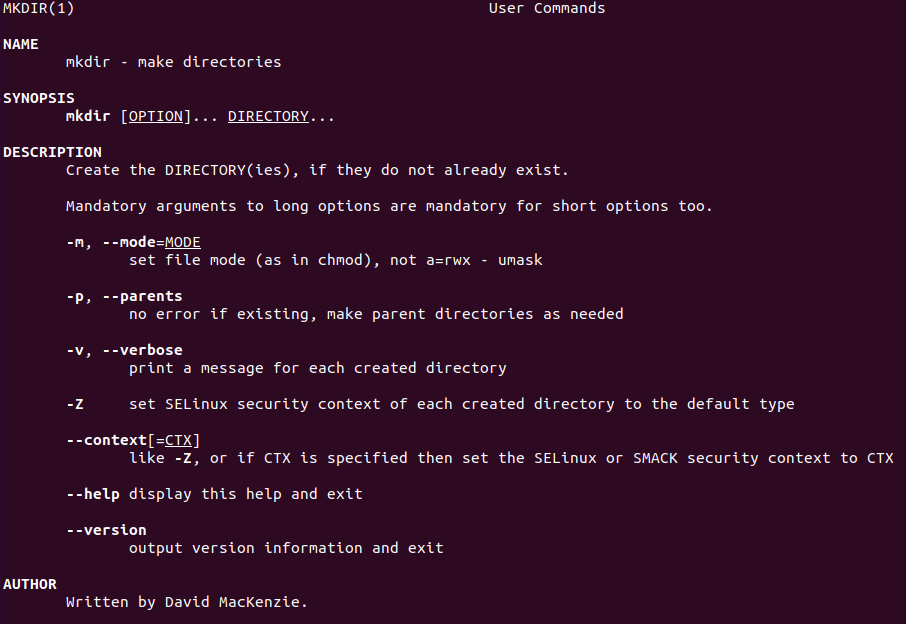
\includegraphics[width=0.9\textwidth]{../figures/shell_man_page_mkdir.png}
	\end{center}
\end{frame}

\begin{frame}
	\frametitle{Command Anatomy: {\tt $--$help} / {\tt -h}}
	Built-in help often a sufficiently quick reminder:
	\begin{center}
		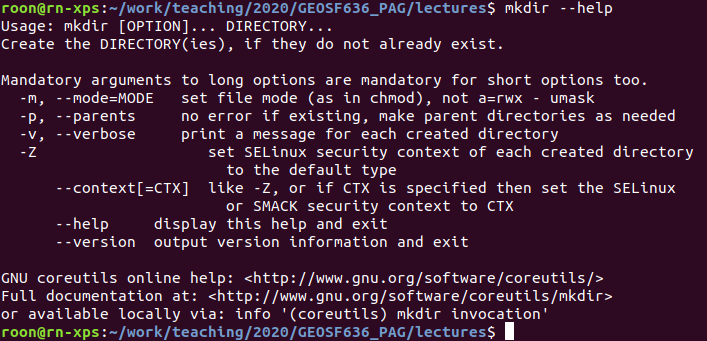
\includegraphics[width=0.9\textwidth]{../figures/shell_help_mkdir.png}
	\end{center}
\end{frame}


\begin{frame}[fragile=singleslide]
	\frametitle{Environment}
	\vspace{-0.25cm}
	\begin{columns}[t]
	\column{0.5\textwidth}
		\begin{center}
			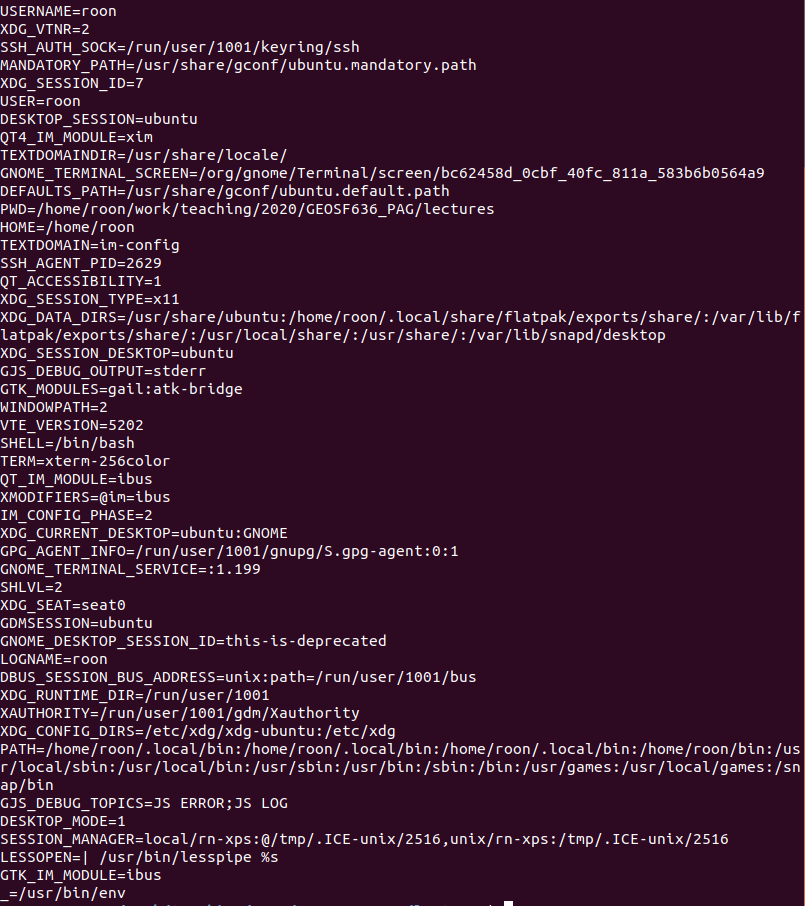
\includegraphics[width=\textwidth]{../figures/env.png}
		\end{center}
	\column{0.5\textwidth}
		\begin{itemize}
		\item {\tt env} command shows values of environment variables
		\item {\tt PATH} probably the most important: specifies directory PATHs where shell tries to find programs
		\end{itemize}
	\end{columns}
	\verb|$> export PATH=/path/to/some/directory:$PATH| (bash)
	\verb|$> setenv PATH /path/to/some/directory:$PATH| (tcsh)
\end{frame}

\begin{frame}[fragile=singleslide]
	\frametitle{Environment - The Path}
	\vspace{-0.25cm}
	\begin{columns}[t]
	\column{0.3\textwidth}
		\begin{center}
			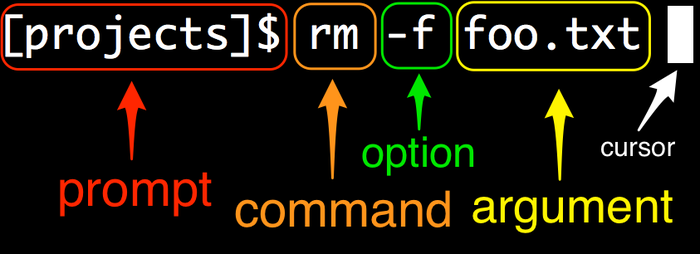
\includegraphics[width=\textwidth]{../figures/shell_cmdline_anatomy.png}
		\end{center}
		\begin{flushright}
			\tiny{\emph{\url{https://www.learnenough.com/command-line-tutorial/basics}}}
		\end{flushright}
	\column{0.7\textwidth}
		\begin{itemize}
		\item Shell tries to execute what you type as a command
		\item Shell maintains a list of all locations of {\bf executable} programs
		\item \verb|PATH| specifies locations of where to find commands / programs 
		\item Shell traverses this list in order. If you got two programs with the same name in different directories, only the one in the first directory will be called. 
		\item Path can be permanently set in config file for shell, e.g. \verb|.bashrc| or \verb|.tcshrc| in home directory\\\vspace{0.25cm}
		\end{itemize}
	\end{columns}
	\verb|$> export PATH=/path/to/some/directory:$PATH| (bash)
	\verb|$> setenv PATH /path/to/some/directory:$PATH| (tcsh)
\end{frame}

\begin{frame}[fragile=singleslide]
	\frametitle{Directories}
	\vspace{-0.25cm}
	\begin{columns}[t]
	\column{0.5\textwidth}
		\begin{center}
			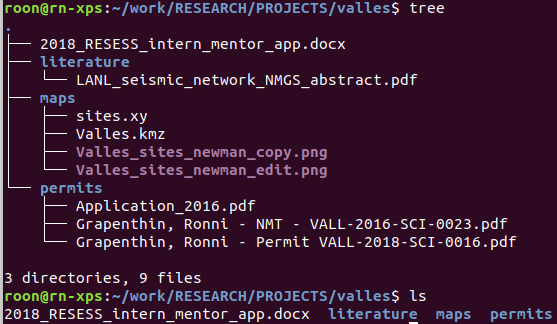
\includegraphics[width=\textwidth]{../figures/shell_directory_tree.png}
		\end{center}
	\column{0.5\textwidth}
		\begin{itemize}
		\item Files and directories are organized in a hierarchial structure
		\item Need to specify names by typing them (no clicking!), tab-completion is useful
		\item Case-sensitive: \verb|case| $\neq$ \verb|CaSe| $\neq$ \verb|CASE|
		\item Special directory symbols:
		\begin{itemize}
			\item \verb|.|  (the current directory)
			\item \verb|..| (the parent directory - one level up in tree)
			\item \verb|~| (the home directory)
		\end{itemize}
		\end{itemize}
	\end{columns}
\end{frame}

\begin{frame}[fragile=singleslide]
	\frametitle{Directory / File Navigation Commands}
	\begin{tabular}{@{\textbullet~}l@{\ }p{2in}}
	  \bfseries \verb|ls|  & list directory contents \\
	  \bfseries \verb|pwd| & {\bf p}rint {\bf w}orking {\bf d}irectory\\
	  \bfseries \verb|cd|  & {\bf c}hange {\bf d}irectory\\
	  \bfseries \verb|cd ..|  & {\bf c}hange {\bf d}irectory one level up\\
	  \bfseries \verb|mkdir test|  & create directory `test'\\
	  \bfseries \verb|mv test dummy| & rename `test' into `dummy'\\
	  \bfseries \verb|touch test-file| & create empty `test-file' or update time stamp if file exists\\
	  \bfseries \verb|mv test-file file2 dummy| & move `test-file' and `file2' into `dummy' directory\\
	  \bfseries \verb|cp dummy/file2 ./| & copy `file2' from `dummy' directory into current directory\\
	  \bfseries \verb|cp -r dummy no-dummy| & copy `dummy' directory and its contents into `no-dummy' directory\\
	  \bfseries \verb|rm -r dummy| & remove non-empty directory `dummy' ({\bf CAREFUL! NO TRASH BIN!})\\
	\end{tabular}
\end{frame}

\begin{frame}[fragile=singleslide]
	\frametitle{Other Useful Commands}
	\begin{tabular}{@{\textbullet~}l@{\ }p{2in}}
	  \bfseries \verb|ls|  	   & list directory contents \\
	  \bfseries \verb|man cmd| & manual page for command `cmd'\\
	  \bfseries \verb|less|    & view a textfile (type `q' to quit)\\
	  \bfseries \verb|head -X| & display first X lines of a file\\
	  \bfseries \verb|tail -X| & display last X lines of a file\\
	  \bfseries \verb|wc file| & count words (-w) or lines (-l) or characters (-c) of a file\\
	  \bfseries \verb|cat file (file2 ...)| & concatenate the contents of files and write out\\
	  \bfseries \verb|sort| & sort contents of a file (even based on columns -k)\\
	\end{tabular}
\end{frame}

\begin{frame}[fragile=singleslide]
	\frametitle{Wildcards}
	\begin{itemize}
		\item Often you want to match multiple files at once, e.g., all files that end in {\tt .py}\\
		\verb|mv *.py listings|
		\item The wildcard `\verb|*|' matches any number of characters:
		\begin{center}
			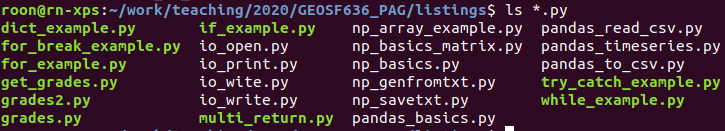
\includegraphics[width=0.9\textwidth]{../figures/shell_wildcards.png}
		\end{center}
		\item Would not match `\verb|numpy|' as it requires a dot before `\verb|py|'
		\item Wildcard recognition and expansion is called `globbing' (stems from `glob' (global) program which initially did this)
	\end{itemize}
\end{frame}

\begin{frame}[fragile=singleslide]
	\frametitle{Wildcards}
		\begin{itemize}
			\item \verb|*| -- Match zero or more characters		
			\item \verb|?| -- Match exactly one character
		\begin{center}
			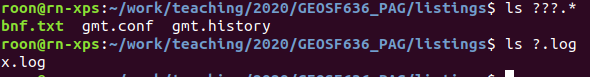
\includegraphics[width=.9\textwidth]{../figures/shell_single_wildcard.png}
		\end{center}
			\item \verb|[a-z]| -- Match lower case letters
			\item \verb|[A-Z]| -- Match upper case letters
			\item \verb|[a-zA-Z]| -- Match upper and lower case letters
			\item \verb|[0-9]| -- Match numbers
		\begin{center}
			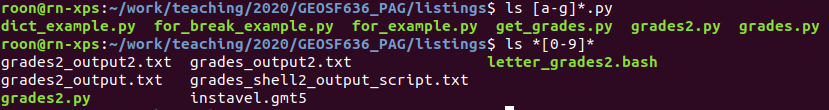
\includegraphics[width=.9\textwidth]{../figures/shell_wildcard_regexp.png}
		\end{center}
		\end{itemize}
\end{frame}


\begin{frame}
	\frametitle{Input/Output Redirection}
	\begin{center}
		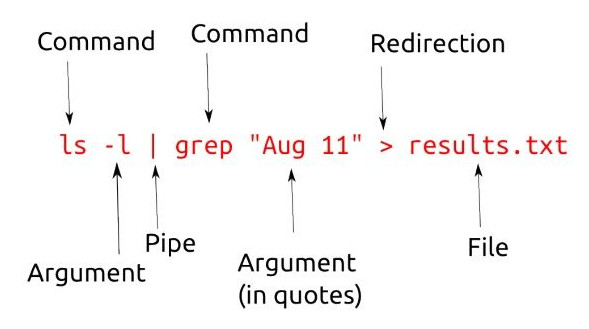
\includegraphics[width=0.5\textwidth]{../figures/shell_long_anatomy.jpg}
	\end{center}
	\begin{flushright}
		\tiny{\emph{The Internet}}
	\end{flushright}
\end{frame}

\begin{frame}[fragile=singleslide]
	\frametitle{Input/Output Redirection}
	\begin{columns}[t]
	\column{0.5\textwidth}
		\begin{itemize}
			\item Many programs designed to take input from {\bf standard input}, write output to {\bf standard output}
			\item By default std-input is keyboard, std-output is the screen
			\item I/O redirection allows you to change that
			\item \verb|<| redirects the input
			\item \verb|>| redirects the output
			\item Can be used at the same time 
		\end{itemize}
	\column{0.5\textwidth}
		\begin{itemize}
			\item Send output to a file:\\
				{\footnotesize \verb/ls *.py > py.lst /\\[10pt]}
			\item Use file as input:\\
				{\footnotesize \verb/sort -r < py.lst/\\[10pt]}
			\item \dots save output to new file\\
				{\footnotesize \verb/sort -r < py.lst > pyr.lst/\\[10pt]}
		\end{itemize}
	\end{columns}
\end{frame}

\begin{frame}
	\frametitle{Piping}
	\begin{center}
		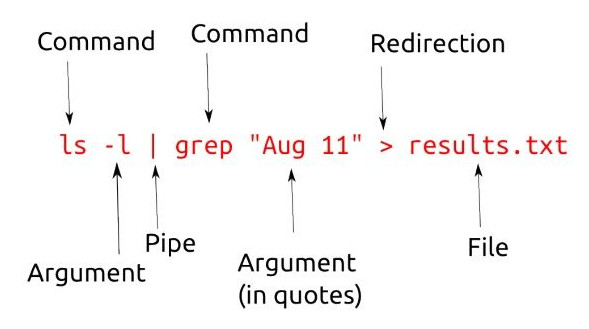
\includegraphics[width=0.5\textwidth]{../figures/shell_long_anatomy.jpg}
	\end{center}
	\begin{flushright}
		\tiny{\emph{The Internet}}
	\end{flushright}
\end{frame}

\begin{frame}[fragile=singleslide]
	\frametitle{Piping}
	 THE INCREDIBLE CONSTRUCT enabling the UNIX philosophy!\\
	\begin{columns}[t]
	\column{0.45\textwidth}
		\begin{itemize}
			\item Use {\bf output} of one program as {\bf input} for another: use the pipe.
			\item Use vertical bar {\tt |} to realize this
			\item Can pipe together as many programs as you like, each needs to read from standard input and write to standard output.
		\end{itemize}
	\column{0.55\textwidth}

		\begin{itemize}
			\item Count files of a given type:\\
				\verb/ls *.py | wc -l/\\[10pt]
			\item Sort listing alphabetically for 9th column\\
				\verb/ls -l | sort -k 9/\\[10pt]
			\item \dots scroll manually\\
				\verb/ls -l | sort -k 9 | less/\\[10pt]
		\end{itemize}
	\end{columns}
\end{frame}

\begin{frame}
	\frametitle{}
\end{frame}

\begin{frame}[fragile=singleslide]
	\frametitle{Everything is Scriptable -- Shell Scripting}
		\begin{itemize}
			\item Do NOT type out / copy'n'paste long series of commands repeatedly
			\item DO bundle sets of commands in an executable script for repeated use
			\item Scripts don't have to be complicated, just need to reliably do something more easily than typing it out
			\item There's no limit to the number of scripts you can write; just remember the names
			\item Here's a script I use to connect to a server (I only need to type \verb|ees.redoubt|, usually, I type \verb|ees.r<tab><enter>|)
		\end{itemize}
		\begin{block}{}
		{\scriptsize
		 \lstinputlisting[language=csh, numbers=none]{../listings/ees.redoubt}
		}
		\end{block}

\end{frame}

\begin{frame}[fragile=singleslide]
	\frametitle{Everything is Scriptable -- Shell Scripting}
		\begin{itemize}
			\item Any series of commands you type at the prompt can be bundles in a script
			\item The shell provides you with variables (e.g., pre-defined \verb|PATH|, or your own)
			\item Flow control allows to write programs (condition testing, loops)
		\end{itemize}
\end{frame}

\begin{frame}[fragile=singleslide]
	\frametitle{Shell Scripting -- Variables}
	\begin{itemize}
	  \item Regular variables (visible just in current shell), spaces are important!!\\
		\verb|set txt = "hello world!"| (tcsh) \\
		\verb|txt="hello world!"| (bash)
	  \item Accessing variables\\
		\verb|echo $txt| (tcsh, bash) \\
	  \item BACKTICKS (execute command in subshell)\\
		\verb|files=`ls *.py`| (bash, works in tcsh too)\\
	  \item Environment Variables (visible in shell and scripts called from this shell)\\
		\verb|setenv PATH /usr/bin| (tcsh)\\
		\verb|export PATH=/usr/bin| (bash)\\
	\end{itemize}
\end{frame}

\begin{frame}[fragile=singleslide]
	\frametitle{Shell Scripting -- Quotes}
	\begin{itemize}
	  \item \verb|'...'| - Single quotes force literal interpretation of what's in the quotes\\
		\vspace{0.25cm}
		\begin{columns}
		\column{0.45\textwidth}
			{\bf tcsh:}\\
			{\scriptsize
			\verb|$>set output = 'I want to say $txt'|\\
			\verb|$>echo $output|\\
			\verb|I want to say $txt|\\
			}
		\column{0.4\textwidth}
			{\bf bash:}\\
			{\scriptsize
			\verb|$>output='I want to say $txt'|\\
			\verb|$>echo $output|\\
			\verb|I want to say $txt|\\
			}		
		\end{columns}
		\vspace{0.25cm}
	  \item \verb|"..."| - Double quotes group words, but variables are still recognized and interpreted\\
		\vspace{0.25cm}
		\begin{columns}
		\column{0.45\textwidth}
			{\bf tcsh:}\\
			{\scriptsize
			\verb|$>set output = "I want to say $txt"|\\
			\verb|$>echo $output|\\
			\verb|I want to say hello world!|\\
			}
		\column{0.4\textwidth}
			{\bf bash:}\\
			{\scriptsize
			\verb|$>output="I want to say $txt"|\\
			\verb|$>echo $output|\\
			\verb|I want to say hello world!|\\
			}
		\end{columns}
	\end{itemize}
\end{frame}

\begin{frame}
	\frametitle{Shell Scripting -- Control Structures (bash only)}
		\vspace{-0.25cm}
		\begin{center}
			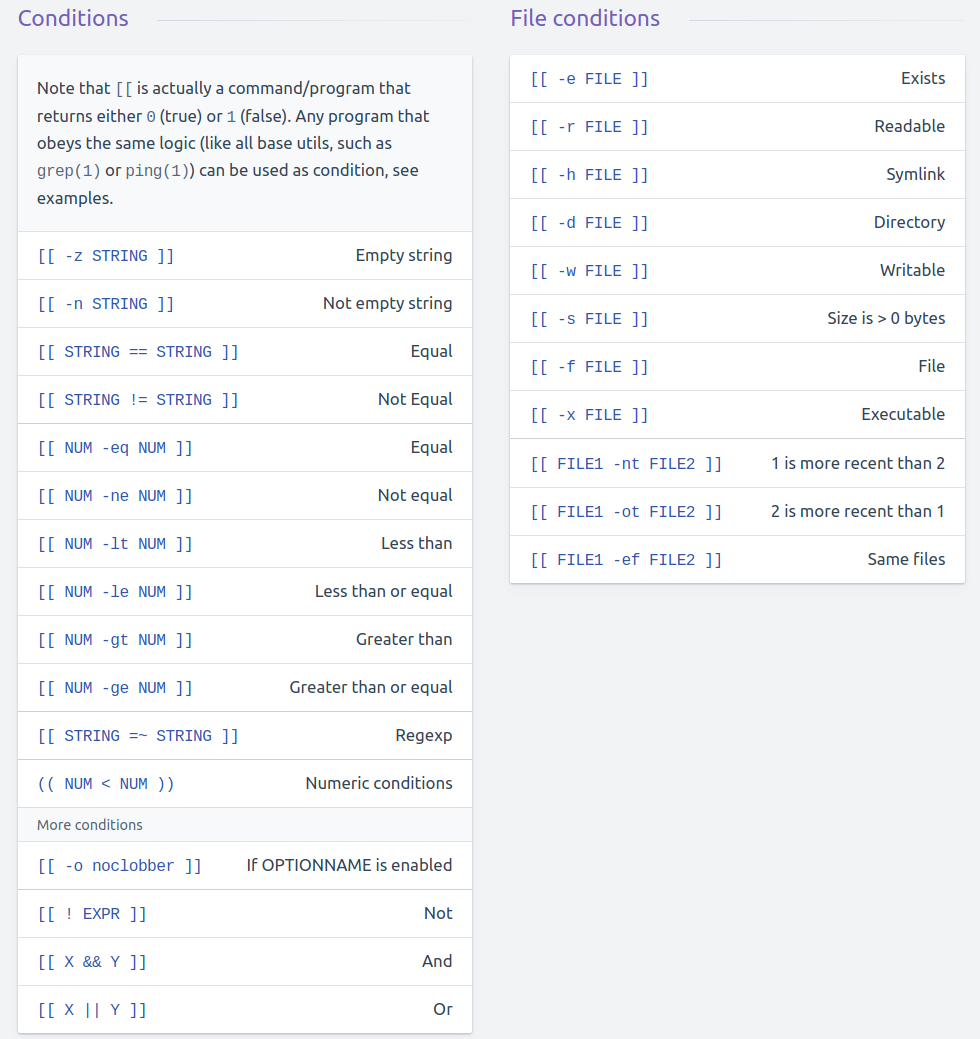
\includegraphics[width=.67\textwidth]{../figures/shell_bash_conditionals.png}
		\end{center}
		\vspace{-1cm}
		\begin{flushright}
			\tiny{\emph{\url{devhints.io/bash}}}
		\end{flushright}
\end{frame}


\begin{frame}
	\frametitle{Shell Scripting -- Control Structures (bash only)}
	\begin{columns}[t]
	\column{0.25\textwidth}
	Conditionals
		\begin{center}
			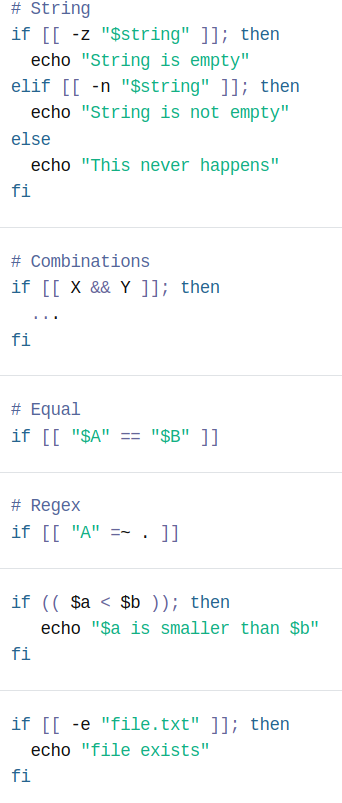
\includegraphics[width=\textwidth]{../figures/shell_bash_if_syntax.png}
		\end{center}
		\vspace{-1cm}
		\begin{flushright}
			\tiny{\emph{\url{devhints.io/bash}}}
		\end{flushright}
	\column{0.7\textwidth}
	\end{columns}
\end{frame}

\begin{frame}
	\frametitle{Shell Scripting -- Control Structures (bash only)}
	\begin{columns}[t]
	\column{0.25\textwidth}
	Conditionals 
		\begin{center}
			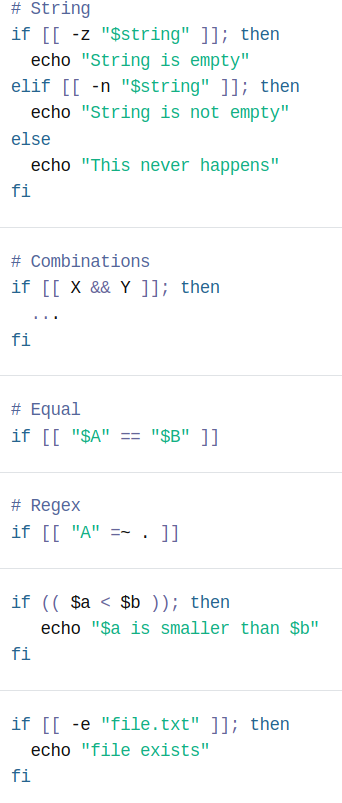
\includegraphics[width=\textwidth]{../figures/shell_bash_if_syntax.png}
		\end{center}
		\vspace{-1cm}
		\begin{flushright}
			\tiny{\emph{\url{devhints.io/bash}}}
		\end{flushright}
	\column{0.7\textwidth}
	Loops
		\begin{center}
			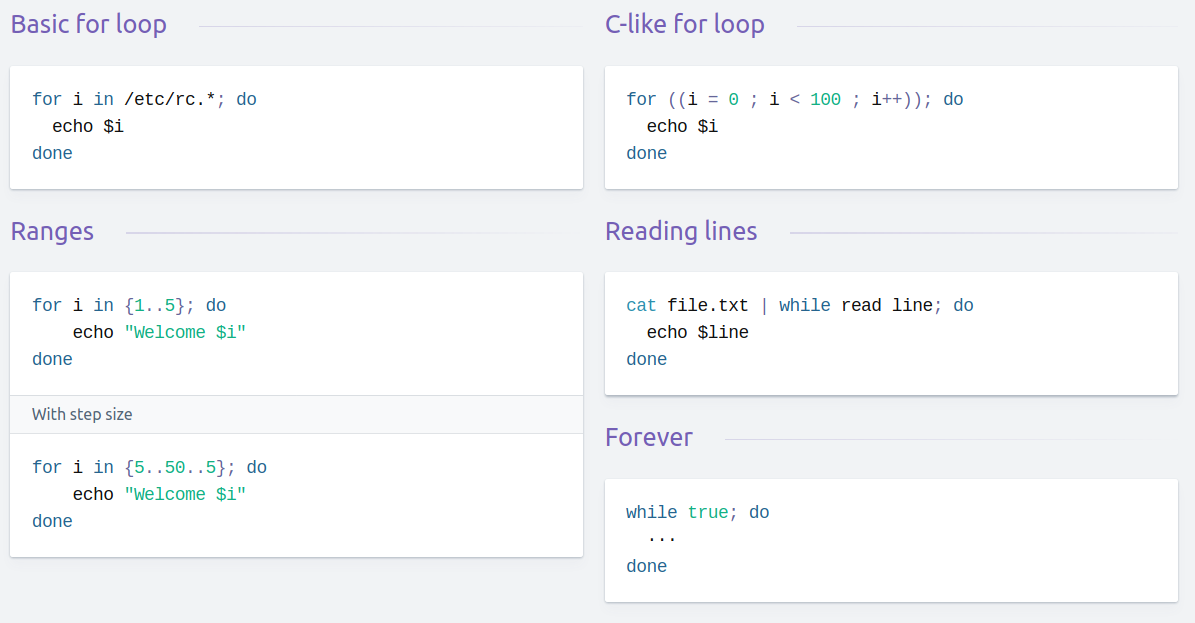
\includegraphics[width=\textwidth]{../figures/shell_bash_loops.png}
		\end{center}
		\vspace{-0.25cm}
		\begin{flushright}
			\tiny{\emph{\url{devhints.io/bash}}}
		\end{flushright}
	\end{columns}
\end{frame}

\begin{frame}[fragile=singleslide]
	\frametitle{Shell Scripting -- Reading Command Line Arguments}
	\begin{itemize}
		\item Shell scripts can take input from the command line
		\item Use special variables \verb|$1,$2,...$n| to get first, second, ... argument
		\item Use special variable \verb|$#| (bash), \verb|$#argv| (tcsh) to get number of arguments
	\end{itemize}
	
		\begin{block}{}
		{\scriptsize
		 \lstinputlisting[language=bash, numbers=none]{../listings/arguments.sh}
		}
		\end{block}

		\begin{block}{}
		{\scriptsize
		 \lstinputlisting[language=bash, numbers=none]{../listings/arguments.out}
		}
		\end{block}

\end{frame}


\end{document}
